\newpage
\section{Backlight}
To goal of having a cheap demonstrator is fully depended on the hardware cost since software is always free to distribute. With this goal in mind we developed a cheap backlight which consists of a fixed PCB panel and a diffusion filter mounted in front of the LED's to spread the light evenly. To inspect the how the luminance of the backlight is captured by the camera, different images of the backlight are plotted as a surface and contour and inspected.\\

\begin{figure}[ht]
	\centering
	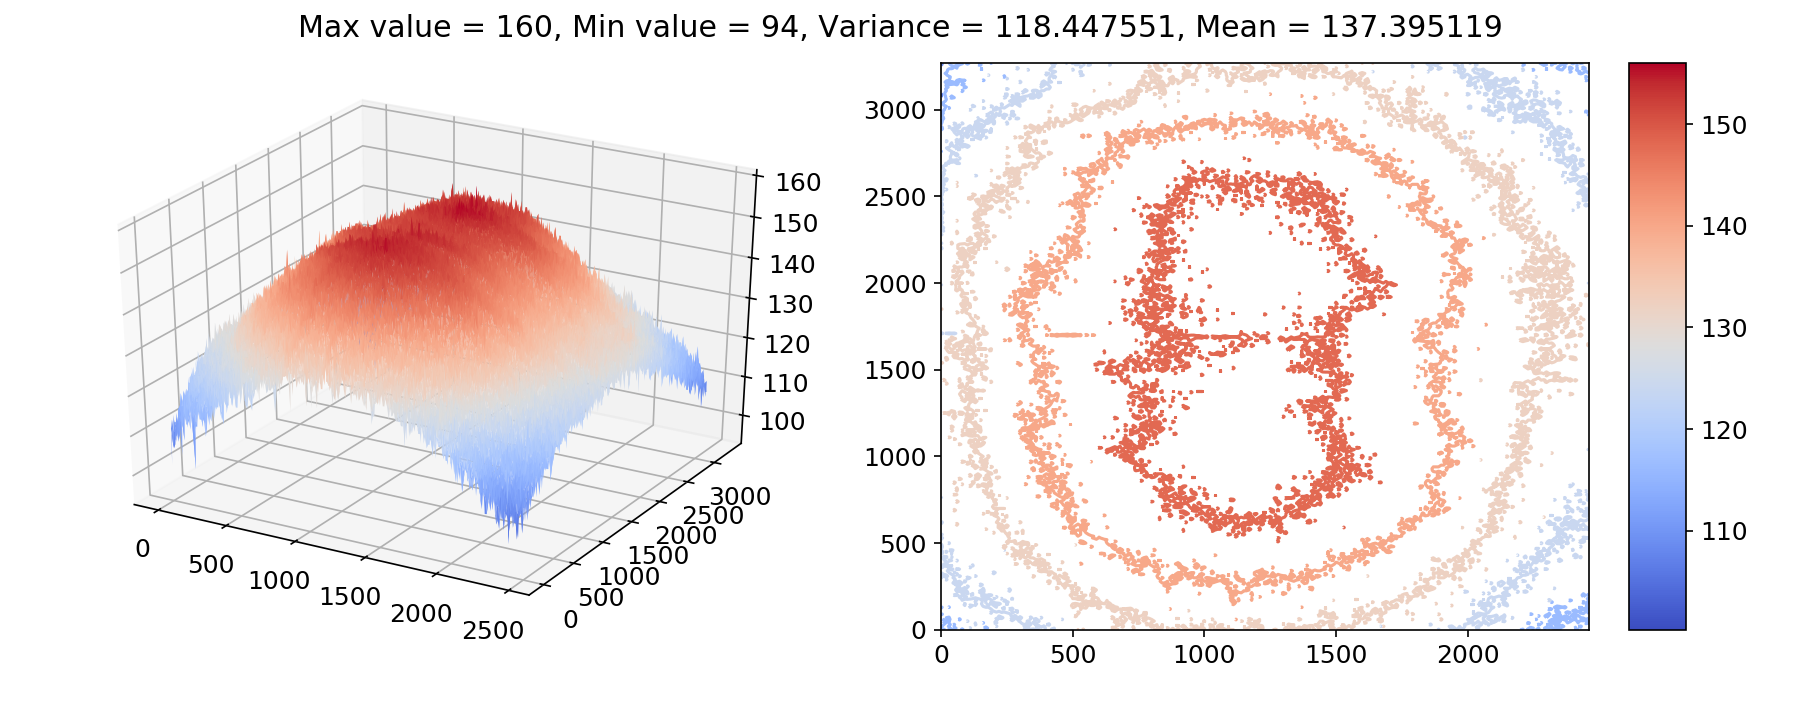
\includegraphics[trim=50 0 0 0,clip,width=1\linewidth]{3-development/backlight/3d0.png}
	\caption{Light source in 3d\label{development:3d0}}
\end{figure} 
Firstly the empty surface without a pattern is analyzed in figure \ref{development:3d0}. In this normal surface we can spot that our edges are less intense as the middle of our backlight. With the gStreamer pipeline auto regulating our brightness to a mean close to 128, we have a maximum value of 160 and a minimum value of 94. 
\begin{figure}[ht]
	\centering
	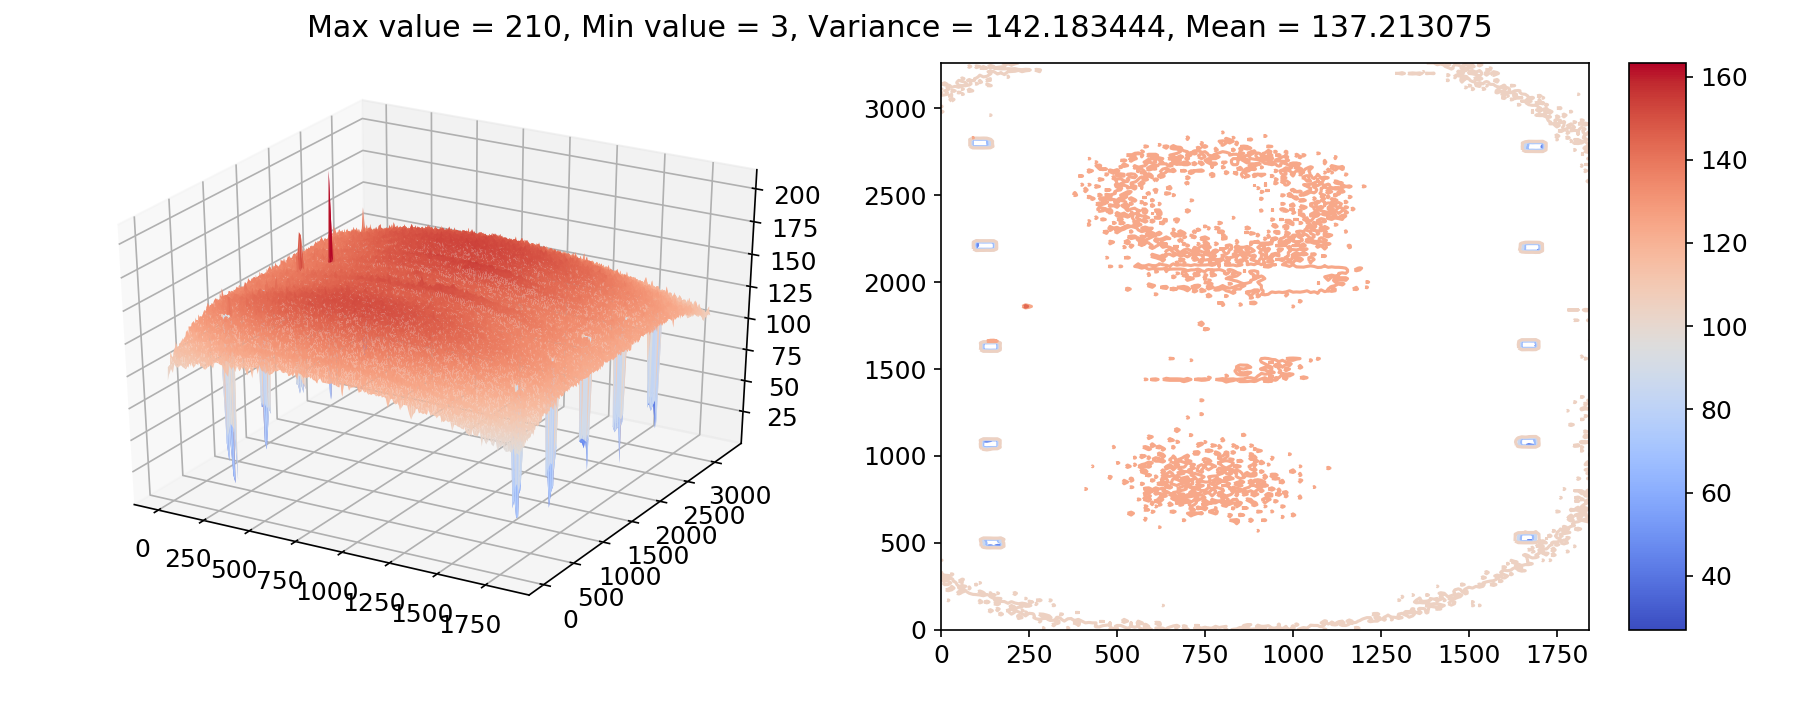
\includegraphics[trim=50 0 0 0,clip,width=1\linewidth]{3-development/backlight/3d1.png}
	\caption{Light source in 3d\label{development:3d1}}
\end{figure} 
The image used for the graphs in \ref{development:3d1} have already the pattern used to measure the spring in them. The pattern consists of five black squares in two rows. Now the lowest point lays in the black squares with the value 3. The maximum value of 210 is an outlier which can be caused by a reflection or not well positioned diffusion filter. The estimated max value is also around if we looking at our plane.
\begin{figure}[ht]
	\centering
	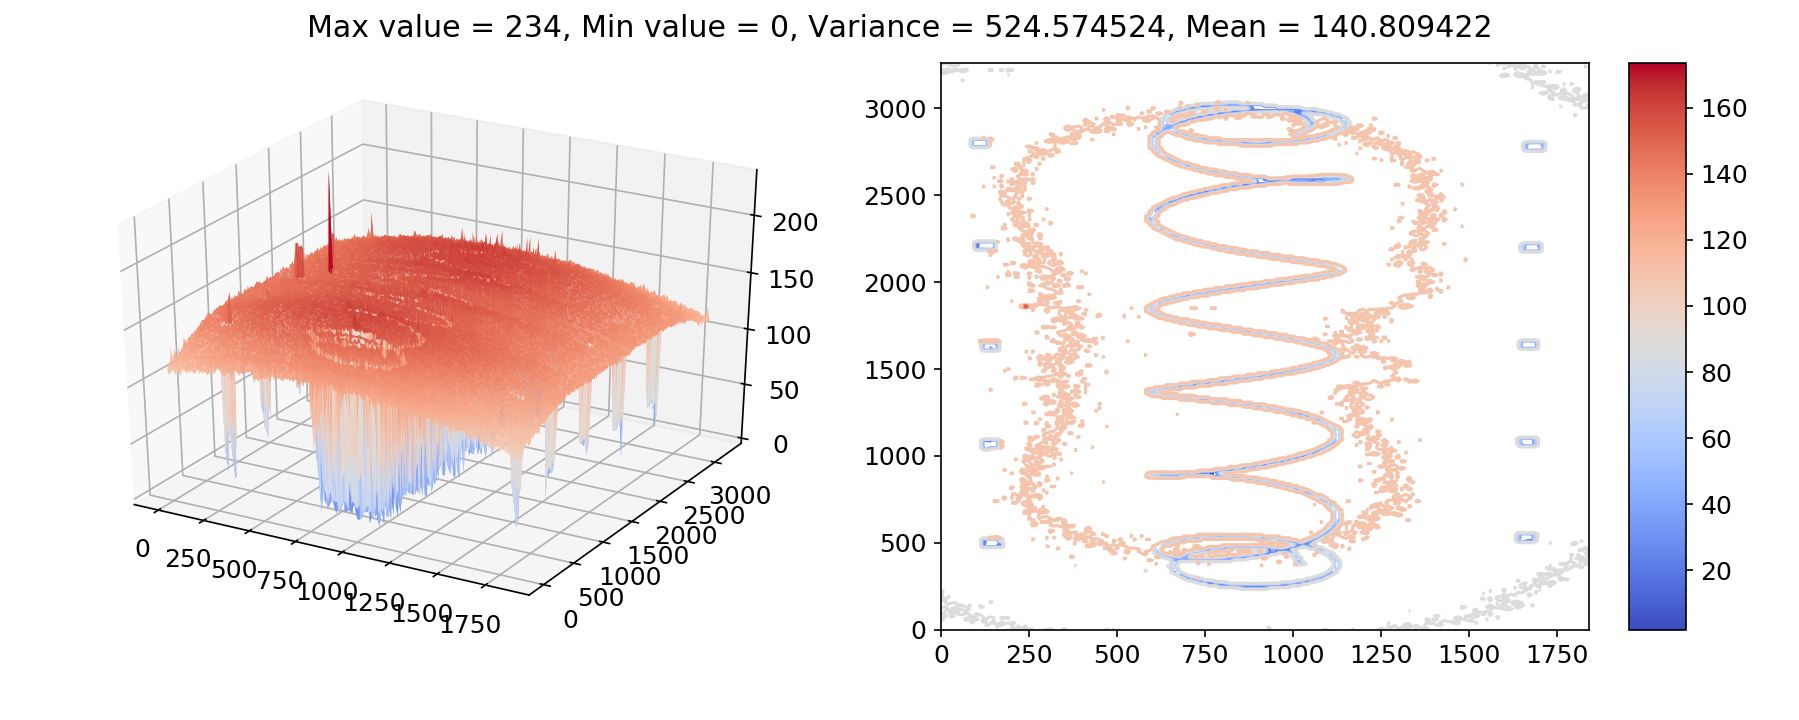
\includegraphics[trim=50 0 0 0,clip,width=1\linewidth]{3-development/backlight/3d4.png}
	\caption{Light source in 3d\label{development:3d4}}
\end{figure} 
In the graph \ref{development:3d4} we can see that the some edges of the spring are very close to the background brightness, a little further to the side. This happens because of the stray light of the backlight illuminating the edge of the spring. Having a round geometry of the sprint the part closer to the backlight and further on the edge off the spring is illuminated more than parts further away. \\
